\documentclass[ddcfooter,nosectionnum]{tudbeamer}
\usepackage{german}
\usepackage{graphicx}
\usepackage{listings}
\usepackage{setspace}
\usepackage{array}
\usepackage{wrapfig}
\usepackage{fontspec}
\usepackage{xltxtra}


\setmainfont{Ubuntu}
\setmonofont{Courier}
\setromanfont{Ubuntu}
\setsansfont{Ubuntu}

\begin{document}

\einrichtung{Fakultät Informatik\hspace{6cm} Institut für Systemarchitektur}
\title[Speicherverwaltung in Linux]{Speicherverwaltung in Linux}
\subtitle{Proseminar Betriebssysteme}
\author{Rebecca Kratsch}

\date{10.05.2013}

\maketitle
	

\begin{frame}
    \frametitle{Inhalt}
	\tableofcontents
\end{frame}

\section{Grundlagen}
\begin{frame} 
    \frametitle{Grundlagen}
    	\begin{itemize}
			\item Physischer Speicher in Seiten strukturiert
			\begin {itemize}
				\item 32-bit Architektur meist 4KB Seiten, 4GB adressierbar
				\item 64-bit Architektur meist 8KB Seiten, 16EB adressierbar
    		\end{itemize}
			\item Virtueller Adressraum je Prozess (auf 32-bit-Maschinen)
			\begin {itemize}
				\item 3GB virtueller Adressraum: Text-, Daten-, BSS-Segment, Stack			\item 1GB: Seitentabellen und andere Informationen des Kerns    			\end{itemize}
    \end{itemize}
\end{frame}


\begin{frame}
	\frametitle{Grundlagen}
    \framesubtitle {Gliederung eines Linux-Prozess-Adressraums}
	
	\begin{minipage}[b]{0.7\textwidth}
			\begin{itemize}
		 		\item Stack:  
				\begin{itemize}
					\item Umgebungsvariablen, Kommandozeile, lokale Variablen
					\item veränderbar
				\end{itemize}  	
				\item Datensegment:  
				\begin{itemize}
					\item initialisierte Daten    
					\item uninitialisierte Daten
				\end{itemize}
				\item Textsegment: 
				\begin{itemize}
					\item Maschinenbefehle
					\item nur lesender Zugriff
					\item feste Größe 
				\end{itemize}
    		\end{itemize}
\end{minipage}
%
\begin{minipage}[b] {0.29\textwidth}
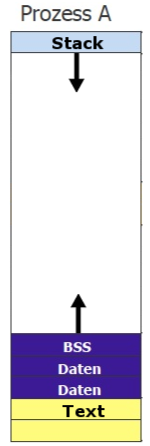
\includegraphics[width=0.58\textwidth]{segmente.png}
\end{minipage} 
\end{frame}

\section{Physischer Speicher}
\begin{frame}
    \frametitle{Physischer Speicher}   
    
	\begin{minipage}[b]{0.7\textwidth} 
		 	\begin{itemize}
				\item 3 Speicherzonen: 
				\begin{enumerate}	 	
					\item ZONE\_DMA 
					\item ZONE\_NORMAL
					\item ZONE\_HIGHMEM
				\end{enumerate}
				\item Arbeitsspeicher 3 Teile: 
				\begin{itemize}
					\item Kern
					\item Speicherzuordnungtabelle
					\item restlicher Anteil: Aufteilung in Seitenrahmen
				\end{itemize}
			\end{itemize}
	\end{minipage}
%
	\begin{minipage}[t]{0.29\textwidth}
		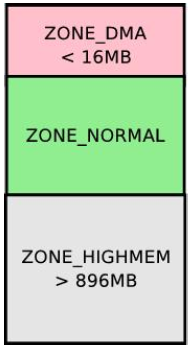
\includegraphics[width=0.6\textwidth]{zonen.png}
	\end{minipage}
\end{frame}

\begin{frame}
	\frametitle{Physischer Speicher}
    \begin{itemize}
    	\item Seitendeskriptoren
        \begin{itemize}
			\item Zeiger auf zugehörigen Adressraum
			\item Typ: \texttt{page}, Name: \texttt{mem\_map}
       	\end{itemize}
		\item Zonendeskriptoren
		\begin{itemize}
			\item Informationen für Speicherausnutzung jeder Zone
			\item Identifizierung freier Arbeitsspeicherbereiche durch
			\texttt{free\_area[]}
		\end{itemize}
		\item Knotendeskriptoren
		\begin {itemize}
			\item zur Differenzierung zwischen physischem Speicher auf verschiedenen Knoten	
			\item Informationen über Speichernutzung und Zonen eines speziellen Knotens
		\end {itemize}			
   	\end{itemize} 

   
       
\end{frame}

\begin{frame}
\frametitle{Physischer Speicher}
\framesubtitle{Mechanismen zur Speicherbelegung}
	\begin{itemize}
		\item<1-4> Speicherallokation unter Nutzung des Buddy-Algorithmus
		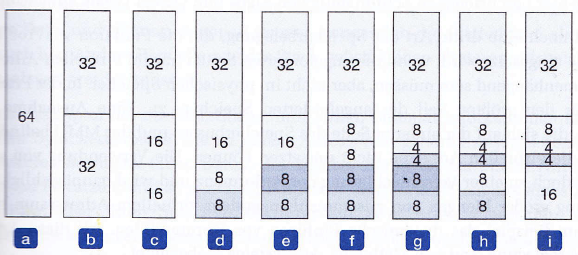
\includegraphics[width=7.5cm]{buddy.png}\\		 
		\visible<1>{\texttt{\tiny Quelle:Tanenbaum, A.; Moderne Betriebssysteme; 3. Auflage}}
		\pause
		
	Problem: interne Fragmentierung\\ 
	\pause
	\item<3-4> Lösung: Slab-Allocator 
	\item<4> Funktion \texttt{vmalloc}	
	\end {itemize}	
	
\end{frame}	


\section{Virtueller Speicher}
\begin{frame}
    \frametitle{Virtueller Adressraum}
    \framesubtitle {Paging in Linux}
    \begin{itemize}
         \item Grundeinheit: Seite
         \item Grundidee / Definition Paging: 
          \end{itemize}
        \begin{quote}
        	\glqq Paging ist ein Speicherverwaltungsverfahren, das auf der Strukturierung  des virtuellen Speichers 	in Seiten und der Strukturierung des realen Speichers in Seitenrahmen beruht. \grqq
         \end{quote}
         \texttt{\tiny Quelle:EHSES, E. u.a. : Betriebssysteme- Ein Lehrbuch mit Übungen zur Systemprogrammierung in UNIX/Linux. 3. Aufl. München: Pearson Studium Verlag, 2005, S.294}
	    
\end{frame}


\begin{frame}
    \frametitle{Virtueller Adressraum}
    \framesubtitle {Paging in Linux}
    \begin{itemize}
    	    \item Beschreibung jedes Bereichs im Kern mit \texttt{vm\_area\_struct}-Eintrag 
   		\begin{itemize}
			\item sortiert und zusammengefasst nach virtueller Adresse\\
			\item enthält Eigenschaften des Bereichs
			\item Angaben über Hintergrundspeicher
    			\item Zugriff auf alle Elemente eines Adressraums via Speicher-Deskriptor
			\begin{itemize}
				\item verkettete Liste
				\item binärer Rot-Schwarz-Baum
			\end{itemize}
   		\end{itemize} 
	\end{itemize}
    
\end{frame}


\begin{frame}
    \frametitle{Virtueller Adressraum}
    \framesubtitle {Paging in Linux}
    \begin{itemize}
         \item Nutzung eines 4-stufigen Paging-Verfahrens         
    	  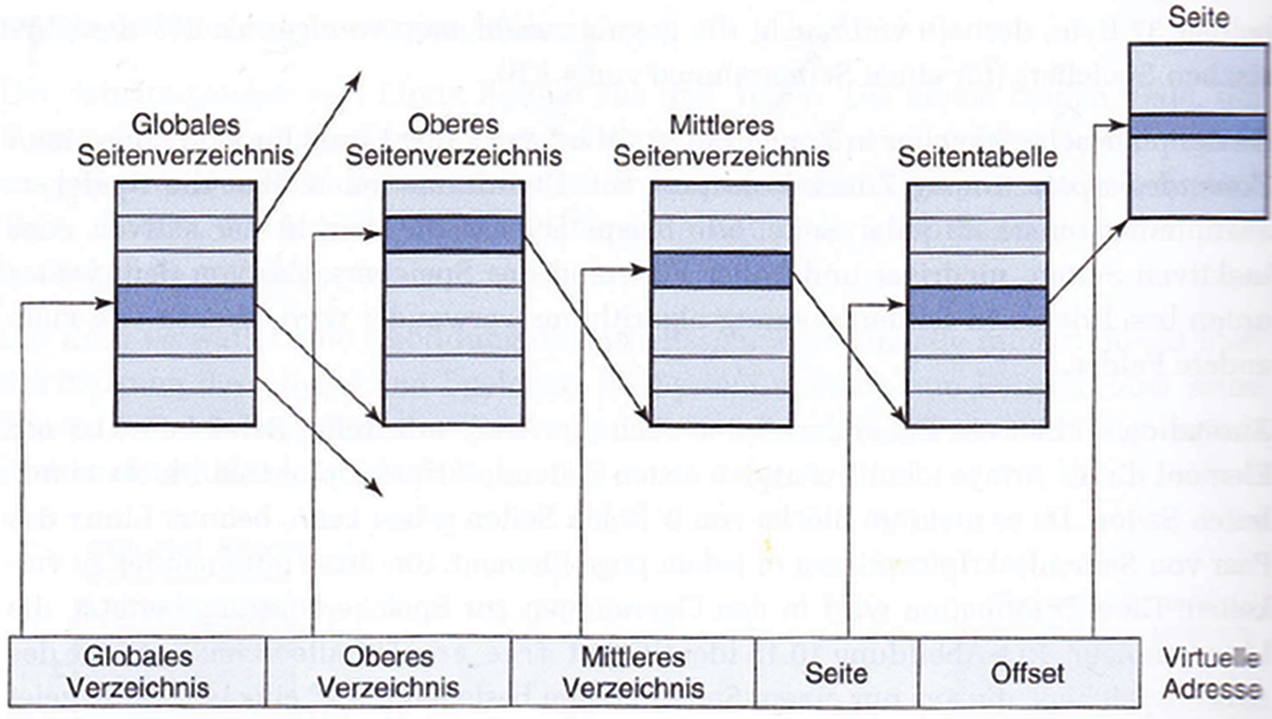
\includegraphics[width=8cm]{vierstufiges.png}\\
    	  \texttt{\tiny Quelle:Tanenbaum, A.; Moderne Betriebssysteme; 3. Auflage}\\
     \end{itemize}
\end{frame}


\begin{frame} 
    \frametitle {Virtueller Adressraum}
    \framesubtitle {Der Seitenersetzungalgorithmus}
    \begin{itemize}
    	\item Realisierung durch Page-Daemon \texttt{kswpd} und \texttt{pdflush}
	 	\item Demand-Paging-System unter Nutzung des Swap-Bereiches
	 	\begin{itemize}
	 		\item Auslagerungspartitionen 
			\item Auslagerungsdateien
		\end{itemize}
		\item Unterscheidung von vier Seitenarten:
		\begin{itemize}
			\item nicht anforderbar
			\item auslagerbar
			\item synchronisierbar
			\item löschbar
		\end{itemize}	
		\item per Page Frame Reclaiming Algorithmus
	\end{itemize}	
\end{frame}

\section{Zusammenfassung}
\begin{frame}
    \frametitle{Zusammenfassung}
    \begin{itemize}
    	\item gradlinig, architekturunabhängig --> hohe Portabilität durch:
		\begin{itemize}
			\item Memory Zones
			\item wenig Verschnitt durch Buddy-Algorithmus und Slab-Allocator 			\item Paging
			\item Seitenersetzungsalgorithmus
		\end{itemize}
	 \end{itemize}
    
\end{frame}


\section{Literatur}
\begin{frame}
    \frametitle{Literatur}
    \begin{itemize}
		\item  Moderne Betriebssysteme \\
        		Andrew S. Tanenbaum - 2010
		\item	 UNIX - Wie funktioniert das Betriebssystem? \\
		Maurice J. Bach - 1991
		\item Betriebssysteme\\
		Ein Lehrbuch mit Übungen zur Systemprogrammierung in UNIX/ Linux \\
		E. Ehses, L. Köhler, P. Riemer, H. Stenzel, F. Victor - 2010	
    \end{itemize}
\end{frame}

\begin{frame}
	
\includegraphics[width= 0.9\textwidth]{br_logo_blau.png}
\end{frame}

\end{document}






